\section{Auswertung}
\label{sec:Auswertung}

\subsection{Magnetfeld von Spulen}
\subsubsection{Kurze Spule}
\label{sec:1}
In diesem Abschnitt wird die gemessene Magnetfeldstärke auf der radialsymmetrischen 
Achse von der kleinen und der großen Spule mit den theoretischen Werten für die 
erwartete Magnetfeldstärke verglichen.
\begin{table}[H]
    \centering
    \caption{Messwerte der kurzen Spule.}
    \label{tab:t1}
    %\sisetup{table-format=1.1, per-mode=reciprocal}
    \begin{tblr}{
        colspec = {S S},
        row{1} = {guard, mode=math},
      }
      \toprule
      \text{x} (\unit{\centi\meter}) & B (\unit{\milli\tesla}) \\
      \midrule
      0   &0.083\\
      1   &0.112\\
      2   &0.154\\
      3   &0.230\\
      4   &0.399\\
      5   &0.727\\
      6   &1.282\\
      7   &1.703\\
      8   &2.053\\
      9   &2.105\\
      10  &1.981\\
      11  &1.589\\
      12  &1.029\\
      13  &0.558\\
      14  &0.332\\
      15  &0.192\\
      16  &0.126\\
      \bottomrule
    \end{tblr}
\end{table}
\noindent In \autoref{tab:t1} sind die aufgenommenen Messwerte der Magnetfeldstärke auf der Achse 
der kleinen Spule zu entnehmen. x ist der Abstand von einem Punkt 5 
\unit{\centi\meter} vor der Spule bis 5 \unit{\centi\meter} hinter der Spule.
Des weiteren sind die Messwerte in \autoref{fig:1} graphisch dargestellt.
\begin{figure}[H]
    \caption{Magnetische Feldstärke auf der Achse der kurzen Spule}
    \label{fig:1}
    \centering
    \includegraphics{"build/plot1.pdf"}
\end{figure}
\noindent In Anbetracht der Tatsache, dass der Eintritt der Hall-Sonde in das Magnetfeld
5 \unit{\centi\meter} von $x = 0$ entfernt liegt und genau so nach dem Austritt
$5$ weitere Messwerte aufgenommen wurden, können wir die restlichen Messwerte, 
die in der Spule aufgenommen wurden, mitteln. Jenes dient dazu, das Magnetfeld 
im Inneren der Spule zu berechnen. Damit wird eine Feldstärke von 
\begin{equation*}
    B_{exp} = \qty{1.63(0.18)}{\milli\tesla}
\end{equation*}
erreicht. Die theoretische Magnetfeldstärke im Inneren der Spule kann mit
\autoref{eqn:4} bestimmt werden. Mit den Werten $I = 1 \unit{\ampere}$,
$n = 100$ und einer Länge von etwa 8 \unit{\centi\meter}
ergibt sich 
\begin{equation*}
    B_{theo} = \qty{1.57e-3}{\tesla} = \qty{1.57}{\milli\tesla}
\end{equation*}

%%%%%%%%%%%%%%%%%%%%%%%%%%%%%%%%%%%%%%%%%%%%%%%%%%%%%%%%%%%%%%%%%%%%%%%%%%%%%%%%%%%%%%%%%%%%%%%%%
\subsubsection{Lange Spule}
Bei der Ermittlung der Magnetfeldstärke in der langen Spule wird genauso
verfahren, wie schon in \autoref{sec:1}.
\begin{table}[H]
    \centering
    \caption{Messwerte der langen Spule.}
    \label{tab:t2}
    %\sisetup{table-format=1.1, per-mode=reciprocal}
    \begin{tblr}{
        colspec = {S S},
        row{1} = {guard, mode=math},
      }
      \toprule
      x (\unit{\centi\meter}) & B (\unit{\milli\tesla}) \\
      \midrule
      0   &0.019\\
      1   &0.041\\
      2   &0.072\\
      3   &0.136\\
      4   &0.253\\
      5   &0.503\\
      6   &0.971\\
      7   &1.544\\
      8   &1.978\\
      9   &2.192\\
      10  &2.279\\
      11  &2.333\\
      12  &2.360\\
      13  &2.379\\
      14  &2.382\\
      15  &2.379\\
      16  &2.368\\
      17  &2.340\\
      18  &2.301\\
      19  &2.231\\
      20  &2.286\\
      21  &2.184\\
      22  &1.965\\
      23  &1.552\\
      24  &0.977\\
      25  &0.519\\
      26  &0.297\\
      27  &0.190\\
      28  &0.133\\
      29  &0.101\\
      30  &0.081\\
      \bottomrule
    \end{tblr}
\end{table}

\begin{figure}[H]
    \caption{Magnetische Feldstärke auf der Achse der langen Spule.}
    \label{fig:1}
    \centering
    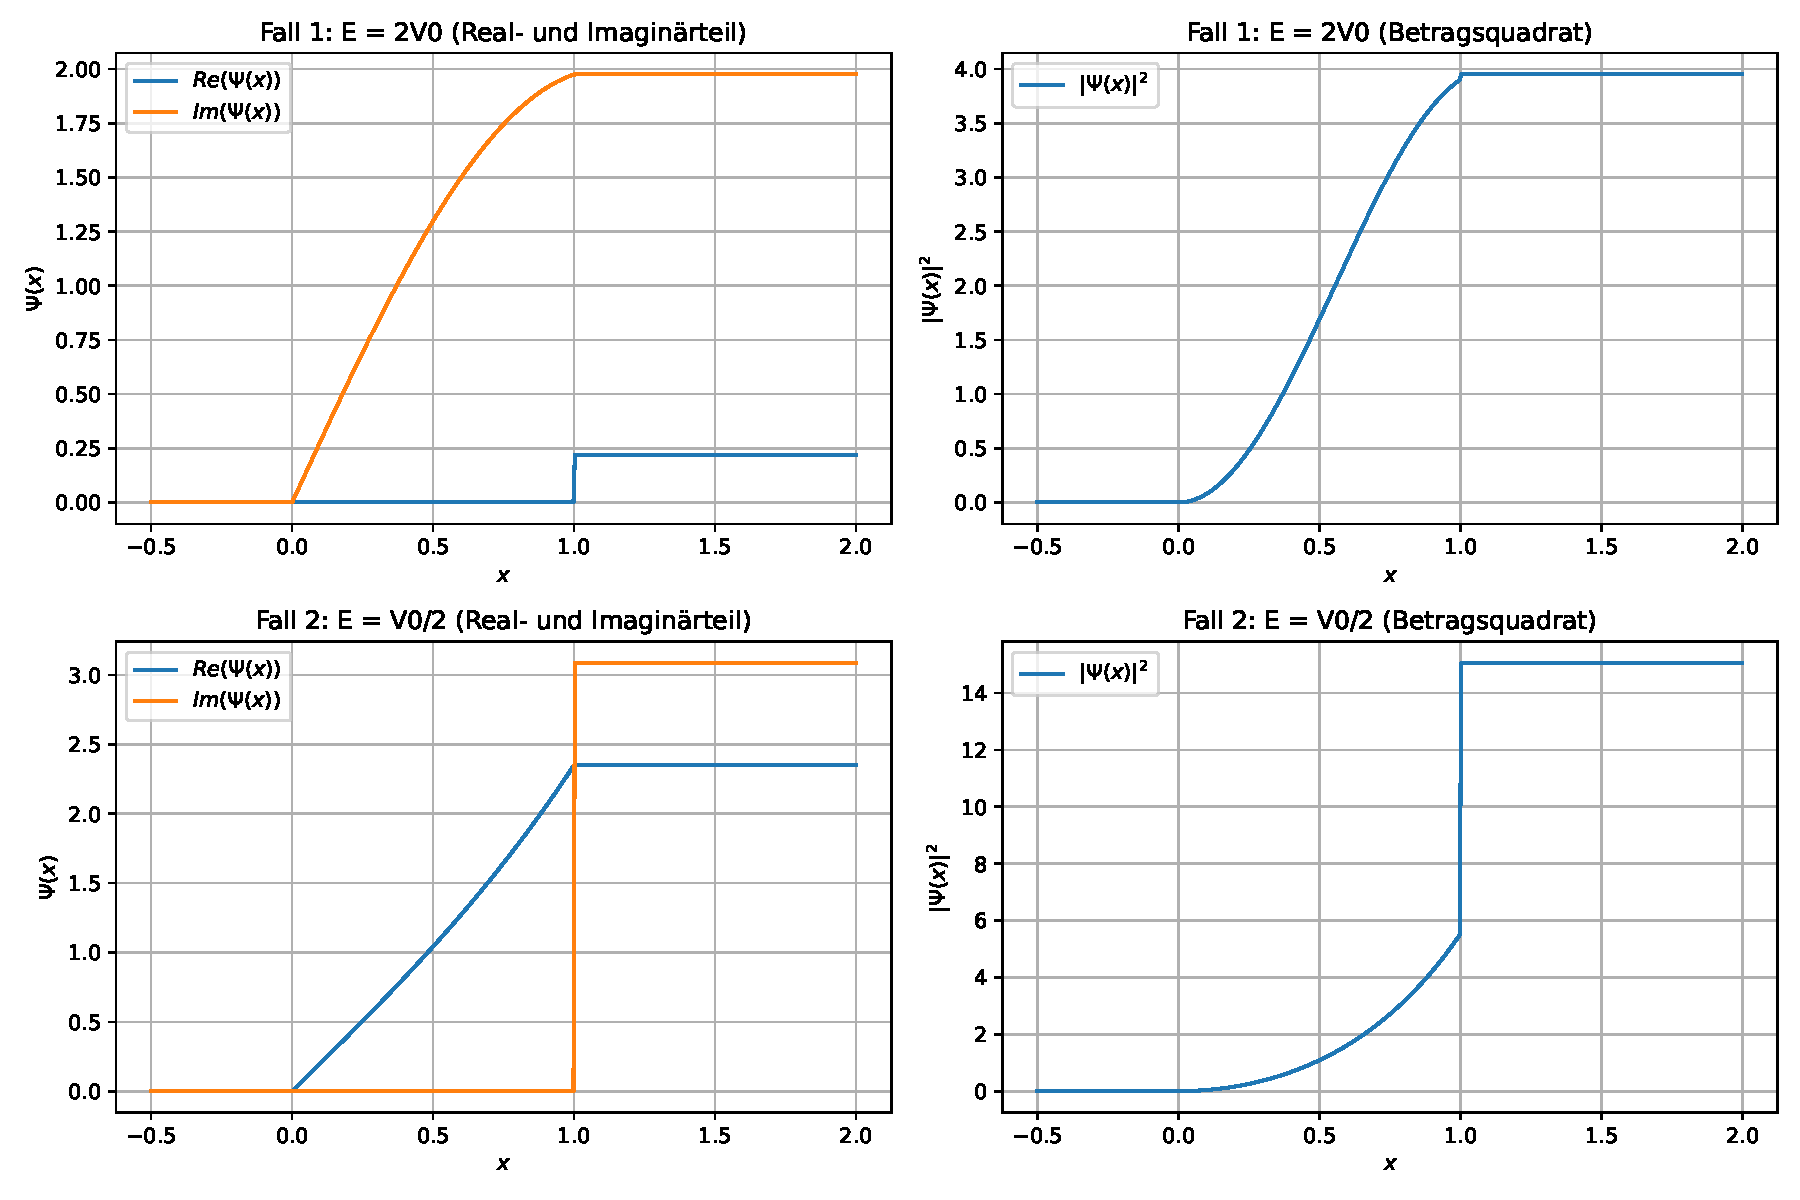
\includegraphics{"build/plot2.pdf"}
\end{figure}
\noindent Aus den Messwerten kann analog zu der kleinen Spule das Magnetfeld
im Inneren gemittelt werden, um einen experimentellen Wert für die 
Magnetfeldstärke im inneren der Spule zu erhalten. Es ergibt sich
\begin{equation*}
    B_{exp,lang} = \qty{1.90(0.13)}{\milli\tesla}.
\end{equation*}
Der Theoretische Wert der Spule mit Länge $l = 19\unit{\centi\meter}$ wird
nach \autoref{eqn:4} bestimmt und beläuft sich auf
\begin{equation*}
    B_{exp,lang} = \qty{1.98e-3}{\tesla} = \qty{1.98}{\milli\tesla}.
\end{equation*}

%%%%%%%%%%%%%%%%%%%%%%%%%%%%%%%%%%%%%%%%%%%%%%%%%%%%%%%%%%%%%%%%%%%%%%%%%%%%%%%%%%%%%%%%%%%%%%%%%%%%%
\subsection{Hysteresekurve}
\begin{table}[H]
    \centering
    \caption{Messwerte Hysteresekurve und resultierendes $H$-Feld.}
    \label{tab:10}
    %\sisetup{table-format=1.1, per-mode=reciprocal}
    \begin{tblr}{
        colspec = {S S S},
        row{1} = {guard, mode=math},
      }
      \toprule
      I (\unit{\ampere}) & B(\unit{\milli\tesla}) & H \unit{\ampere\meter}\\
      \midrule
      0 &  1   & 0.      \\
    1  & 90    & 701.   \\
    2  & 260   & 1402.   \\
    3  & 390   & 2104.   \\
    4  & 479   & 2805.   \\
    5  & 540   & 3507.   \\
    4  & 516   & 2805.   \\
    3  & 483   & 2104.   \\
    2  & 430   & 1402.   \\
    1  & 308   & 701.  \\
    0  & 122   & 0.      \\
    -1 & -80   & -701.   \\
    -2 & -258  & -1402   \\
    -3 & -395  & -2104   \\
    -4 & -482  & -2805   \\
    -5 & -540  & -3507   \\
    -4 & -515  & -2805   \\
    -3 & -483  & -2104   \\
    -2 & -429  & -1402   \\
    -1 & -305  & -701.   \\
    0  & -117  & 0.      \\
    1  & 79    & 701.   \\
    2  & 259   & 1402.   \\
    3  & 392   & 2104.   \\
    4  & 479   & 2805.   \\
    5  & 340   & 3507.   \\
    \bottomrule
    \end{tblr}
\end{table}

Über die aufgenommenen Messwerte der Magnetfeldstärke im Luftspalt der Ringspule soll hier 
die Sättigungsmagnetisierung, Remanenz und Koerzitivkraft bestimmt werden.
\begin{figure}[H]
    \caption{Hysteresekurve}
    \label{fig:3}
    \centering
    \includegraphics{"build/plot3.pdf"}
\end{figure}
\noindent Die Werte der Remananz, sowie der Sättigungswert können der Tabellle 
\autoref{tab:10} entnommen werden.
\begin{align*}
    B_{R1} =& 122 \unit{\milli\tesla}\\
    B_{R2} =& -117 \unit{\milli\tesla}\\
&\\
    H_{S1} =& 540 \unit{\mega\ampere\per\meter}\\
    H_{S2} =& -540 \unit{\mega\ampere\per\meter}\\
\end{align*}

\noindent Die Koerzitivkraft kann mit einer linearen Ausgleichsgeraden durch
die jeweils zwei nächsten Messpunkte zum Nulldurchgang der magnetischen
Feldstärke $B$ bestimmt werden. Es werden die Punkte
$(0:123),(-1:-80)$ sowie $(0:-117),(1:79)$ verwendet. Daraus ergibt sich:
\begin{align*}
    H_{K} =& 0.344 \unit{\kilo\ampere\per\meter}\\
    H_{K} =& 0.324 \unit{\kilo\ampere\per\meter}\\
\end{align*}

\noindent Die differentielle relative Permeabilität kann mit \autoref{eqn:10}
und den Messwerte aus \autoref{tab:10} berechnet werden. 
\begin{equation}
    \mu_{diff} = \frac{1}{\mu_0} \frac{B_2 - B_1}{H_2 - H_1}
\end{equation}
\noindent Durch Einsetzen der Werte ergibt sich die differentielle magnetische
Permeabilität zu
\begin{equation}
    \mu_{diff} = \frac{1}{\mu_0} \frac{0.00539 \unit{\tesla}}{3507 \unit{\ampere\per\meter}} = 1.223
\end{equation}





%%%%%%%%%%%%%%%%%%%%%%%%%%%%%%%%%%%%%%%%%%%%%%%%%%%%%%%%%%%%%%%%%%%%%%%%%%%%%%%%%%%%%%%%%%%%%%%
\subsection{Helmholtz-Spulen}
Den Tabellen \autoref{tab:12} und \autoref{tab:11} sind die Werte für die Magnetfeldstärke auf der 
Symetrieachse eines Helmholzspulenpaares einmal für große und einmal für kleine 
Abstände der Spulen zu entnehmen. $x$ in $\unit{\milli\meter} $ ist dabei der
Abstand vom linken Ende der Skala zu der Hall-Sonde. Um die Darstellung und den Vergleich mit der 
Theoriekurve zu vereinfachen wurde die $x$-Skala so verschoben, dass der Nullpunkt
jeweils in der Mitte der beiden Spulen liegt.

\begin{table}[H]
    \centering
    \caption{Gemessene Magnetfeldstärke im Abstand $x$ vom inneren Rand der linken Spule aus (also ohne Verschiebung) für Spulenabstand $d = 8\unit{\centi\meter}$.}
    \label{tab:12}
    %\sisetup{table-format=1.1, per-mode=reciprocal}
    \begin{tblr}{
        colspec = {S S },
        row{1} = {guard, mode=math},
      }
      \toprule
      x (\unit{\milli\meter}) & B(\unit{\milli\tesla}) \\
      \midrule
      10 & 1.200\\
      11 & 1.199\\
      12 & 1.199\\
      13 & 1.197\\
      14 & 1.196\\
      15 & 1.195\\
      16 & 1.195\\
      17 & 1.193\\
      18 & 1.191\\
      19 & 1.190\\
      20 & 1.195\\
      21 & 1.196\\
      22 & 1.196\\
      23 & 1.197\\
      24 & 1.197\\
      25 & 1.198\\
      90  &-0.808\\
      100 &-0.664\\
      110 &-0.537\\
    \bottomrule
    \end{tblr}
\end{table}

\begin{table}[H]
    \centering
    \caption{Gemessene Magnetfeldstärke im Abstand $x$ vom inneren Rand der linken Spule aus (also ohne Verschiebung) für Spulenabstand $d = 20\unit{\centi\meter}$.}
    \label{tab:11}
    %\sisetup{table-format=1.1, per-mode=reciprocal}
    \begin{tblr}{
        colspec = {S S },
        row{1} = {guard, mode=math},
      }
      \toprule
      x (\unit{\centi\meter}) & B(\unit{\milli\tesla}) \\
      \midrule
      1  &-0.713\\
      2  &-0.606\\
      3  &-0.509\\
      4  &-0.429\\
      5  &-0.369\\
      6  &-0.330\\
      7  &-0.308\\
      8  &-0.304\\
      9  &-0.318\\
      10 &-0.350\\
      11 &-0.400\\
      12 &-0.474\\
      13 &-0.562\\
      14 &-0.666\\
      15 &-0.770\\
      21 &-0.665\\
      23 &-0.434\\
      25 &-0.267\\
    \bottomrule
    \end{tblr}
\end{table}
\noindent Die Messwerte sind in \autoref{fig:10} für $d = 20 \unit{\centi\meter}$
und in \autoref{fig:11} für $d = 8 \unit{\centi\meter}$ zusammen mit einer nach
\autoref{eqn:2} berechneten Theoriekurve für den entsprechenden Abstand und
einer Windungsanzahl von $100$, sowie einem Radius von $\qty{62.5}{\milli\meter}$ 
und $\mu_0 = 4 \pi \cdot 10^{-7}\unit{\newton\per\ampere\squared}$
graphisch dargestellt.

\begin{figure}
    \caption{Magnetfeldstärke Spulenpaar $19\unit{\centi\meter}$ Abstand.}
    \label{fig:10}
    \centering
    \includegraphics{"build/plot4.pdf"}
\end{figure}

\begin{figure}
    \caption{Magnetfeldstärke Spulenpaar $8\unit{\centi\meter}$ Abstand.}
    \label{fig:11}
    \centering
    \includegraphics{"build/plot5.pdf"}
\end{figure}